\chapter{Dark Mode Implementation}

\section{Context}

Many users today configure their \acf{OS} and browsers to use dark mode by default, making dark interfaces an increasingly expected feature in modern applications. This trend is particularly noticeable among younger user segments, including the Rakuten France 2026's \acf{OKRs} growth target, where dark UI experiences are often preferred.

To address these expectations, this task focuses on introducing dark mode support across the frontend ecosystem.

The first step consists of extending \texttt{next-common} to provide the required dark mode foundation, including theme management, design token adaptation, and component compatibility. Once this shared foundation is available, dark mode is progressively integrated into the different consuming \texttt{*-fo} applications.

As an introductory task within the frontend platform, this work requires interaction with multiple parts of the monorepo ecosystem, including themes, design tokens, reusable components, Storybook, build pipelines, and downstream application integration.

\section{Phase 01: Research \& Technical Planning}

\subsection{Dark Mode Definition, Importance, and Challenges}

\paragraph{Definition:}

Dark mode is a user interface theme that replaces traditional light backgrounds with darker color palettes while adapting text, components, and visual elements to maintain readability and accessibility.

\paragraph{Importance:}

The adoption of dark mode has become an important aspect of modern \acs{UX} for several reasons:

\begin{itemize}
    \item \textbf{User preferences:} Many users configure their \acs{OS} and browsers to use dark mode by default, expecting applications to automatically adapt to their system preferences.

    \item \textbf{Improved \acs{UX}:} Dark interfaces provide a more comfortable viewing experience, particularly in low-light environments, and can help reduce visual discomfort during prolonged usage.

    \item \textbf{Modern \acs{UX} standards:} Supporting dark mode enables applications to meet current design expectations and provide a consistent experience across modern platforms, including e-commerce applications.

    \item \textbf{Energy efficiency:} Dark mode can reduce power consumption on OLED and AMOLED displays, as darker pixels require less energy to illuminate.
\end{itemize}

\paragraph{Challenges:}

Though, it's important to adapt dark mode across a large-scale frontend ecosystem, the process presents several technical challenges:
\begin{itemize}
    \item \textbf{State management in a micro-frontend architecture:} Maintaining a consistent theme state across multiple independent frontend applications requires a shared approach to theme detection, synchronization, and persistence.
    
    \item \textbf{Image adaptation:} Many e-commerce product images are designed with light backgrounds. Ensuring proper visibility and contrast on dark surfaces requires careful handling of images, backgrounds, and visual assets.
    
    \item \textbf{Component and design consistency:} All shared components, design tokens, and UI elements must support both themes while preserving accessibility, readability, and visual consistency across applications.
\end{itemize}

\subsection{Technical decisions}

\begin{enumerate}
    \item \textbf{State management:}
    \begin{itemize}
        \item \textbf{Options considered:} React Context, Zustand, Redux.
        \item \textbf{Choice:} \textbf{React Context} with \texttt{AppThemeContext} to manage the theme state, as the application only requires a simple global theme value.
    \end{itemize}

    \item \textbf{CSS strategy:}
    \begin{itemize}
        \item \textbf{Options considered:} \texttt{.dark-mode} class, \texttt{data-theme} attribute, MUI-only styling.
        \item \textbf{Choice:} The \texttt{data-theme} \acs{HTML} attribute, providing a centralized and flexible way to control themes through \acs{JS} \acs{DOM} manipulation.
    \end{itemize}

    \item \textbf{Persistence:}
    \begin{itemize}
        \item \textbf{Options considered:} sessionStorage, localStorage, cookies.
        \item \textbf{Choice:} \textbf{\texttt{localStorage}} with the \texttt{theme} key storing \texttt{light} or \texttt{dark}, ensuring the user's preference is preserved across sessions without server-side storage.
    \end{itemize}

    \item \textbf{MUI and CSS variables synchronization:}
    \begin{itemize}
        \item \textbf{Options considered:} Duplicated palettes, MUI v7 CssVarsProvider, CSS variable-based JS tokens.
        \item \textbf{Choice:} \ac{JS} tokens are mapped to CSS variables using \texttt{var(- -*)} references with \texttt{cssVariables: true} in \texttt{createTheme} of \texttt{CssVarsProvider}, ensuring consistency between MUI components and global styles.
    \end{itemize}

    \item \textbf{SSR and hydration:}
    \begin{itemize}
        \item \textbf{Choice:} The \texttt{data-theme} attribute is applied inside the \texttt{<html>} tag before React hydration, ensuring that the initial render matches the user's preferred theme and preventing visual inconsistencies.
    \end{itemize}
\end{enumerate}

\subsection{Syncing MUI theme with global CSS variables}

The codebase mixes \textbf{MUI \lstinline|sx| / \lstinline|styled|} and \textbf{plain CSS modules} components. To keep them in sync we set a single source of truth (CSS variables) and let both worlds resolve to it, here is the steps to do so:

\begin{enumerate}
    \item Define separate light and dark CSS palettes through global CSS variables, using the \texttt{data-theme} attribute as a selector: \texttt{:root[data-theme='light']} for the light mode and \texttt{:root[data-theme='dark']} for the dark mode.
    \item Redefine JS color tokens to reference the CSS variables using \texttt{var(--*)}, ensuring that both MUI components and CSS modules resolve to the same color values.
    \item Implement the MUI theme using \texttt{CssVarsProvider} with \texttt{cssVariables: true} (new in MUI v7) and feeds \texttt{palette.mode} from the runtime.
    \item \texttt{ThemeContextProvider} toggles \texttt{document.documentElement.dataset.theme} between 'light' and 'dark', which flips the CSS variables globally, which in turn re-tints every MUI component and every CSS module simultaneously.
\end{enumerate}

\begin{figure}[H]
    \centering
    \begin{minipage}[t]{0.48\textwidth}
        \begin{lstlisting}[caption={custom-light-variables.css}]
:root, :root[data-theme="light"],
.light-mode {
  --palette-mode: "light";
  --inverse-mode: "dark";

  --white-900: "#FFFFFF";
  --black-900: "#000000";
}
        \end{lstlisting}
    \end{minipage}
    \hfill
    \begin{minipage}[t]{0.48\textwidth}
        \begin{lstlisting}[caption={custom-dark-variables.css}]
:root[data-theme="dark"],
.dark-mode {
  --palette-mode: "dark";
  --inverse-mode: "light";
  
  --white-900: "#000000";
  --black-900: "#FFFFFF";
}
        \end{lstlisting}
    \end{minipage}
\label{fig:css-variables-palettes}
\end{figure}
\begin{figure}[h]
    \centering
    \begin{minipage}[t]{0.24\textwidth}
    \end{minipage}
    \hfill
    \begin{minipage}[t]{0.48\textwidth}
        \begin{lstlisting}[caption={colorPalette.ts}]
export const colorPalette = {
  paletteMode: 'var(--palette-mode)',
  inverseMode: 'var(--inverse-mode)',

  white900: 'var(--white-900)',
  black900: 'var(--black-900)',
};
        \end{lstlisting}
    \end{minipage}
    \hfill
    \begin{minipage}[t]{0.24\textwidth}
    \end{minipage}
\label{fig:color-palette}
\end{figure}

\subsection{Resolving the Flash Of Unstyled Content Problems}

One of the main challenges when implementing dark mode in \acs{SSR}-based applications is preventing the Flash Of Unstyled Content (FOUC). Without a pre-hydration mechanism, the browser initially renders the default light theme before React hydrates the page and applies the user's preferred dark theme, resulting in a noticeable visual flash. To address this issue, a \textbf{synchronous inline script} is injected in the document \texttt{<head>} to set the \texttt{data-theme} attribute before the CSS is parsed and before the page is rendered, ensuring that the correct theme is applied from the first paint.

\begin{figure}[h]
\centering
\begin{lstlisting}[caption={ThemeInitScript.tsx}]
'use client';
import React from 'react';
export const ThemeInitScript = () => (
  <script id="theme-init"
    dangerouslySetInnerHTML={{
      __html: ` document.documentElement.dataset.theme =
          localStorage.getItem("theme") ||
          (window.matchMedia("(prefers-color-scheme: dark)").matches
            ? "dark" : "light"); `, }} /> );
\end{lstlisting}
\label{fig:theme-init-script}
\end{figure}

\subsection{POC Implementation with MUI 5 and MUI 7}

A small POC was implemented to validate the dark mode technical approach across MUI v5 and MUI v7. The main findings are:

\begin{itemize}
    \item \textbf{MUI v5:} Does not provide native CSS Variables support, requiring a custom solution to synchronize \ac{JS} themes with \acs{CSS} variables.
    
    \item \textbf{MUI v7:} Introduces built-in \texttt{cssVariables: true} support in \texttt{createTheme}, simplifying theme synchronization and customization.
    
    \item \textbf{Migration:} The upgrade from MUI v5 to MUI v7 was included as part of the dark mode implementation.
\end{itemize}

\section{Phase 02: Technical Implementation in \texttt{next-common}}

\subsection{Migration to MUI v7}

The first step of the implementation was upgrading the MUI ecosystem from v5 to v7 to benefit from the native CSS variables support introduced in the latest version.

\begin{figure}[h]
    \centering
    \begin{minipage}{0.5\textwidth}
        \begin{lstlisting}[caption={MUI dependencies update}]
"@mui/material":         "^7.3.8",
"@mui/icons-material":   "^7.3.8",
"@mui/system":           "^7.3.8",
"@mui/material-nextjs":  "^7.3.8",
"@mui/x-date-pickers":   "^7.29.4"
        \end{lstlisting}
    \end{minipage}
\end{figure}

The migration required updating theme-related imports and adapting components to the new MUI APIs. The main changes included:

\begin{itemize}
    \item Updating theme utilities to use \lstinline|@mui/material/styles| instead of deprecated APIs such as \lstinline|@mui/styles|.
    \item Updating components affected by breaking changes introduced in MUI v7, such as replacing the previous \lstinline|Grid| implementation with \lstinline|GridLegacy| where required.
\end{itemize}

\subsection{Setting \textbf{global-css} as the source of truth}

To support dark mode consistently across the ecosystem, color definitions were moved from \ac{JS} objects to CSS variables managed by the \texttt{global-css} package.

Two palettes were introduced, light and dark palette presented in Figure~\ref{fig:css-variables-palettes}.

This approach allows both MUI components and CSS modules to consume the same design tokens without duplicating theme logic.

The \lstinline|colorPalette.ts| file was updated to reference CSS variables names instead of static hex values as in Figure~\ref{fig:color-palette}.

\subsection{{ThemeContextProvider}}

The theme management across all consuming applications is centralized in the shared \texttt{ThemeContextProvider} inside the \texttt{next-common/mui} package.

Its responsibilities are:

\begin{itemize}
    \item Detecting the user's preferred theme using system preferences.
    \item Persisting manual selections using \lstinline|localStorage|.
    \item Updating the global \lstinline|data-theme| attribute.
    \item Providing the active theme palette to MUI through \texttt{ThemeProvider}.
\end{itemize}

As a result, applications using the shared MUI provider automatically gain dark mode support, Phase 03.

\subsection{\texttt{globalTheme} with CSS variables}

The MUI theme configuration was updated to enable CSS variables:

\begin{lstlisting}
const theme = {
  cssVariables: true,
  palette: {
    mode: paletteMode,
  },
};
\end{lstlisting}

All palette values were replaced with CSS variable references, allowing MUI components and custom CSS styles to automatically adapt when the active theme changes.

\textbf{Note:} Some components requiring transparency were migrated from dynamic color manipulation to predefined overlay variables, since MUI's \lstinline|alpha()| utility does not directly support CSS variables.

\subsection{Storybook integration}

Storybook was updated to support theme switching through a global toolbar control.

The integration includes:

\begin{itemize}
    \item A theme selector allowing switching between light and dark modes.
    \item Loading global CSS variables inside the Storybook environment.
    \item Wrapping stories with the shared \texttt{ThemeContextProvider}.
\end{itemize}

\subsection{Header \& Footer adaptation}

The shared \texttt{Header} and \texttt{Footer} components were adapted to support dark mode by replacing hardcoded colors with the new CSS variable-based design tokens. Due to the complexity of these components, additional adjustments were required to ensure proper contrast, readability, and visual consistency across both themes.

The main changes included:
\begin{itemize}
    \item Replacing static colors with dynamic palette variables for backgrounds, texts, borders, and icons.
    \item Updating logos and SVG assets to support theme-dependent colors.
    \item Ensuring navigation elements, menus, links, and interactive components remain accessible in both light and dark modes.
\end{itemize}

Figures~\ref{fig:header-light} and~\ref{fig:header-dark} demonstrate the Header component in both the light and dark themes. 

\begin{figure}[H]
    \centering
    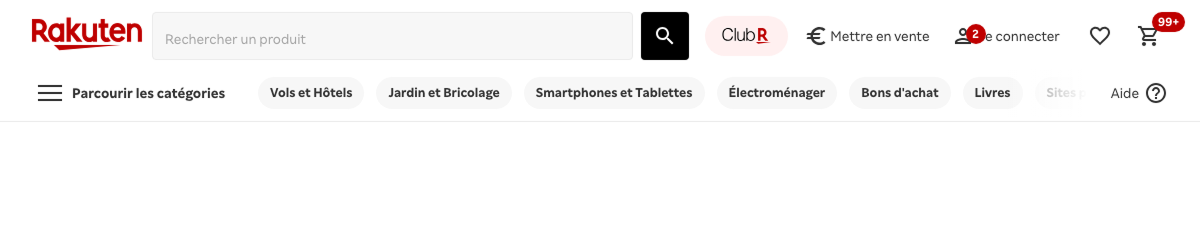
\includegraphics[width=1\textwidth]{../assets/dark_mode/header_light.png}
    \caption{Header component in light mode from Storybook.}
    \label{fig:header-light}
\end{figure}

\begin{figure}[H]
    \centering
    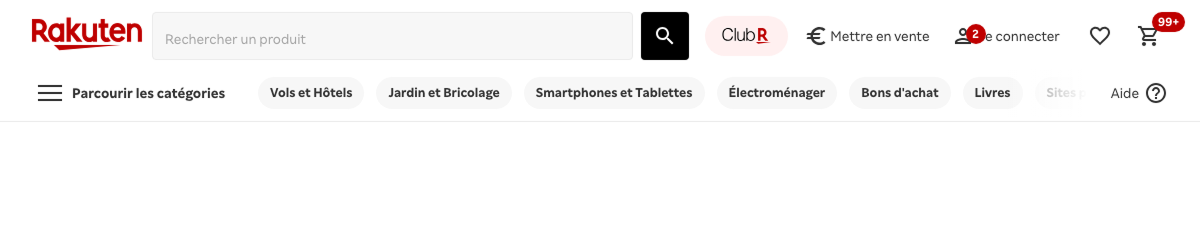
\includegraphics[width=1\textwidth]{../assets/dark_mode/header_dark.png}
    \caption{Header component in dark mode from Storybook.}
    \label{fig:header-dark}
\end{figure}

Figures~\ref{fig:footer-light} and~\ref{fig:footer-dark} illustrate the Footer adaptation to both the light and dark themes.

\begin{figure}[H]
    \centering
    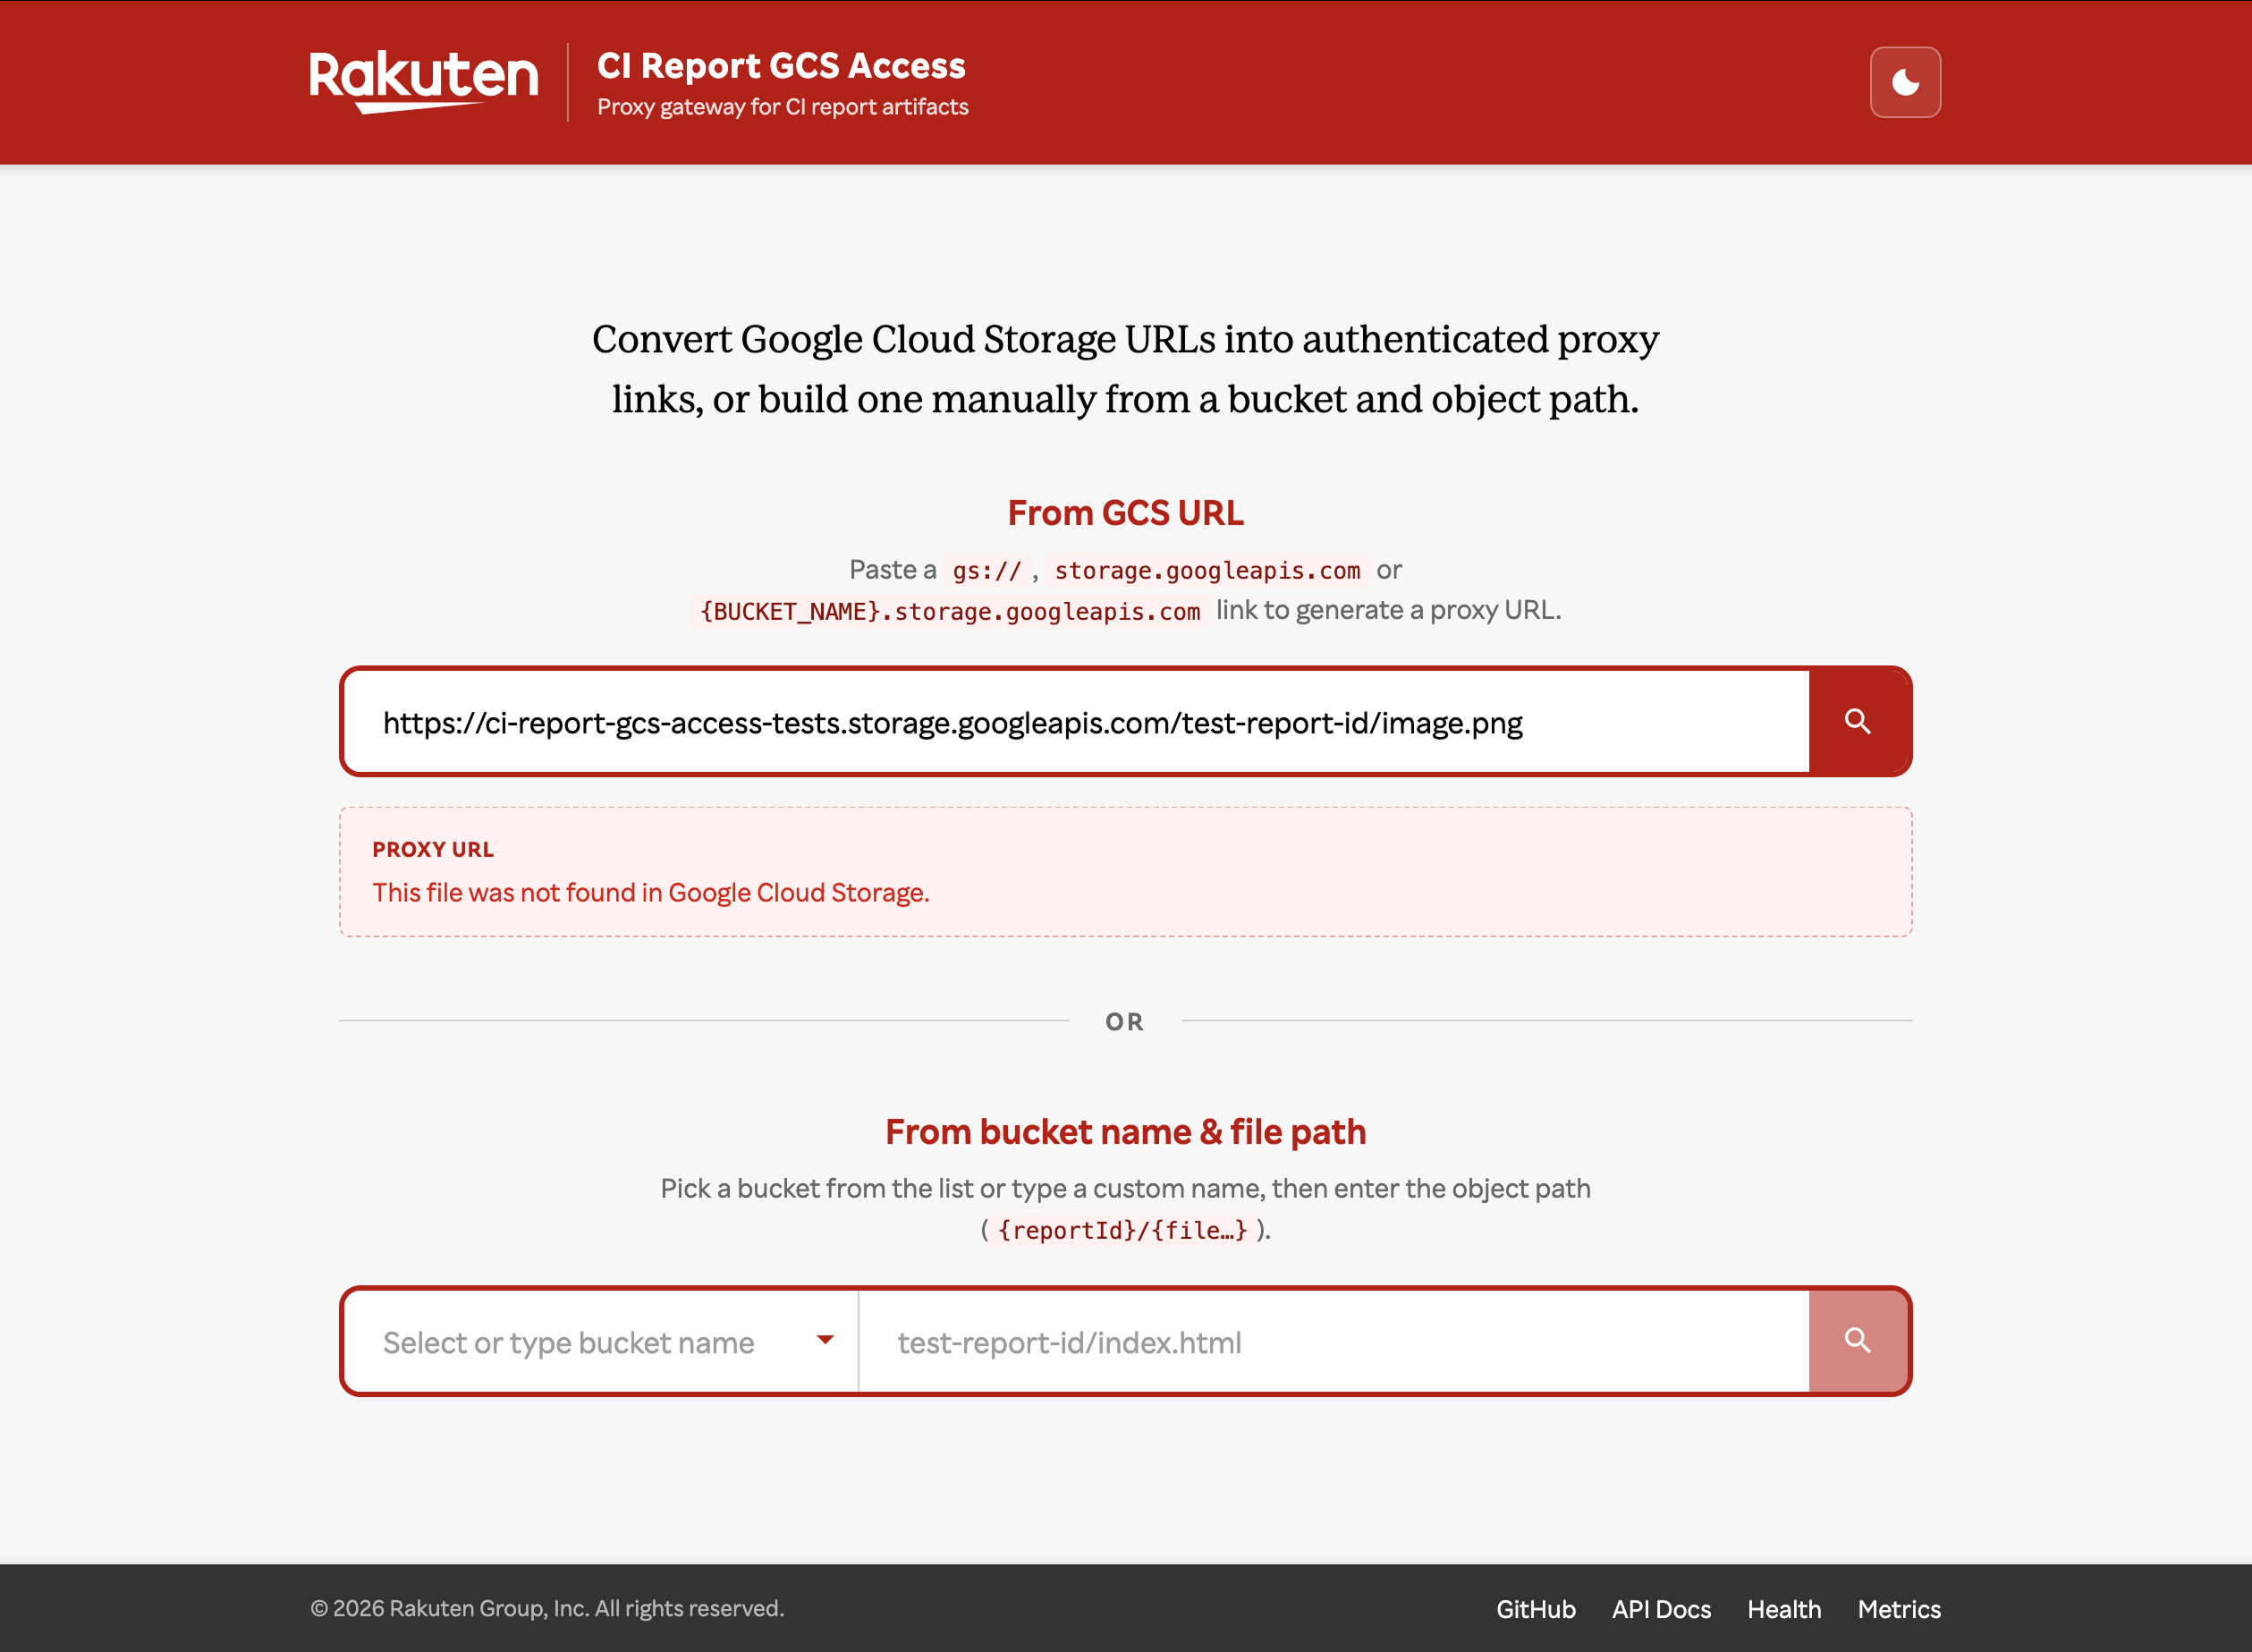
\includegraphics[width=1\textwidth]{../assets/dark_mode/footer_light.png}
    \caption{Footer component in light mode from Storybook.}
    \label{fig:footer-light}
\end{figure}

\begin{figure}[H]
    \centering
    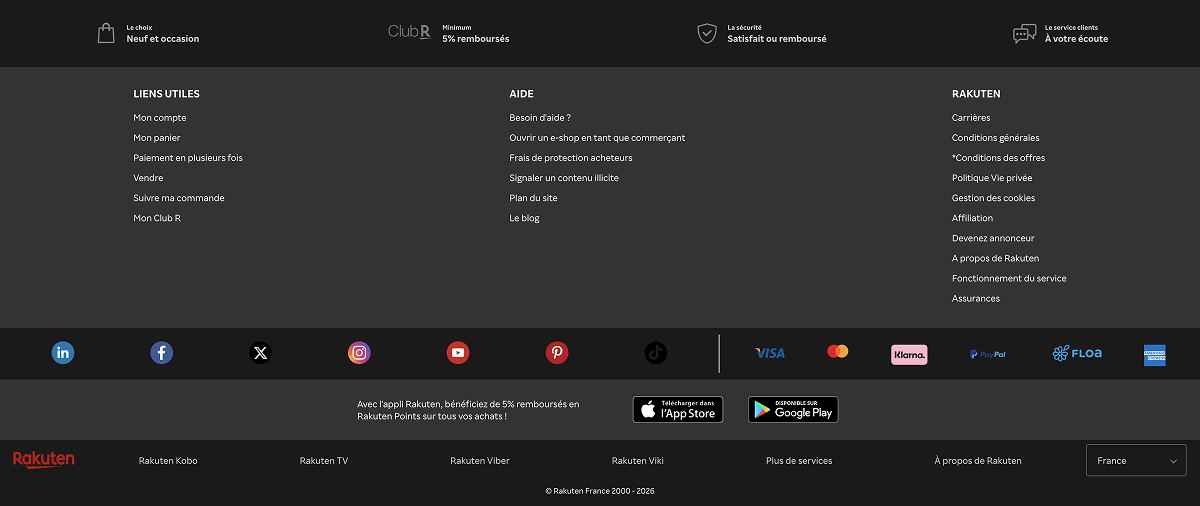
\includegraphics[width=1\textwidth]{../assets/dark_mode/footer_dark.png}
    \caption{Footer component in dark mode from Storybook.}
    \label{fig:footer-dark}
\end{figure}

\subsection{Circular Dependency Resolution}

To provide a shared foundation for dark mode across the frontend ecosystem, the \texttt{global-css} package was transformed into a standalone package responsible for exposing both CSS variables and \ac{JS} design tokens.

Previously, color tokens were defined inside the \lstinline|mui| package. However, this approach created a dependency issue because some packages, such as \lstinline|shared-svg|, needed access to the same color tokens while already being consumed by \lstinline|mui|. Moving the color palette directly to \lstinline|global-css| was necessary to avoid creating a circular dependency between packages.

The dependency issue was resolved by applying the following changes:

\begin{itemize}
    \item Moving \lstinline|colorPalette| from \lstinline|@rakutenfrance/mui| to \lstinline|@rakutenfrance/global-css|, making it available as a shared dependency.
    \item Updating packages such as \lstinline|shared-svg| to consume color tokens from \lstinline|global-css| instead of depending on \lstinline|mui|.
    \item Keeping \lstinline|global-css| as a low-level package with no dependency on UI components, preventing reverse dependencies.
\end{itemize}

The package was also updated to expose compiled artifacts instead of relying on raw source files. It now provides:

\begin{itemize}
    \item Compiled CSS files containing the light and dark theme variables.
    \item JavaScript exports containing the CSS variable-based color tokens.
    \item Proper package metadata (\lstinline|main|, \lstinline|types|, and \lstinline|exports|) to support consumption by downstream applications.
\end{itemize}

This new architecture establishes \lstinline|global-css| as the single source of truth for theme tokens, allowing all consuming applications and shared components to use the same color system and ensuring consistent dark mode behavior across the frontend ecosystem.

\subsection{Adding dark mode to the rest of the ecosystem}

After establishing the dark mode foundation in \lstinline|next-common|, the remaining applications and packages in the frontend ecosystem were progressively updated to consume and integrate the new theme infrastructure.

The main adaptations included:

\begin{itemize}
    \item Updating \lstinline|colorPalette| imports to use \lstinline|@rakutenfrance/global-css|, ensuring that all packages consume the centralized CSS variable-based design tokens.
    
    \item Wrapping Next.js applications with \lstinline|ThemeContextProvider| to provide a consistent theme state management mechanism, handle user preferences, and synchronize the active theme across the application.
    
    \item Replacing hardcoded colors with dynamic CSS variables, allowing shared components and application-specific styles to automatically adapt to both light and dark themes.
    
    \item Updating visual assets such as logos, SVGs, and images to support theme-dependent rendering and maintain proper contrast and visibility in dark mode.
\end{itemize}

These changes ensure that all applications built on top of the shared frontend ecosystem benefit from a consistent dark mode experience while minimizing duplicated theme logic and maintenance overhead.

\subsection{Testing and Quality Assurance}

To validate the dark mode implementation, Storybook was used as a visual testing environment for the different packages and shared components. Each component was reviewed in both light and dark modes to ensure that the visual appearance, accessibility, and behavior remained consistent across themes.

The validation process focused on:

\begin{itemize}
    \item Verifying color contrast, readability, and accessibility requirements in both themes.
    \item Ensuring that components dynamically adapt when switching between light and dark modes.
    \item Detecting visual inconsistencies caused by remaining hardcoded colors or unsupported assets.
\end{itemize}

\subsection{Building and Deployment}

Once the implementation was completed and validated, the updated packages were built and published to the internal GitHub Package Registry, making the new dark mode capabilities available to downstream applications consuming the shared frontend ecosystem.

Additionally, the packages were published to Chromatic to enable visual regression testing and provide an updated component documentation environment. This ensures that future changes can be automatically compared against the validated light and dark mode states.

\section{Phase 03: Rollout to \texttt{fo-apps}}

After completing the dark mode foundation in \texttt{next-common}, the next step consists of progressively integrating the new theme infrastructure into the consuming frontend applications.

The objective of this phase is to ensure that all applications built on top of the shared ecosystem benefit from the same theme management mechanism, design tokens, and component compatibility without duplicating dark mode logic.

\subsection{Application migration steps}

Each downstream application consuming the \texttt{next-common} packages follows the same integration process:

\begin{enumerate}
    \item \textbf{Upgrade dependencies:} Applications are migrated to the compatible MUI v7 ecosystem and updated shared packages versions to consume the new dark mode capabilities.

    \item \textbf{Update theme-related imports:} Existing imports are adapted to follow the MUI v7 API conventions.

    \item \textbf{Expose theme switching:} Application interfaces such as headers or user menus can use \lstinline|useThemeContext()| to provide users with a theme toggle functionality.

    \item \textbf{Replace application-level hardcoded colors:} Local styles and components are updated to consume the shared CSS variable-based design tokens instead of static color values.

    \item \textbf{Adapt visual assets:} Images, logos, and SVG components are reviewed and updated to ensure correct visibility and contrast in both themes.
\end{enumerate}


\subsection{Application validation}

After integration, each application is validated to ensure consistent behavior across themes.

The validation process includes:

\begin{itemize}
    \item Checking the correct initialization of the selected theme after page refresh.
    \item Verifying theme persistence across user sessions.
    \item Testing main user flows in both light and dark modes.
    \item Ensuring that application-specific components follow the shared design token system.
\end{itemize}

This rollout strategy allows applications to progressively adopt dark mode while relying on the centralized implementation provided by \texttt{next-common}, reducing duplication and ensuring a consistent user experience across the frontend ecosystem.

Figures~\ref{fig:buy-fo-gift-card-light} and~\ref{fig:buy-fo-gift-card-dark} illustrate the transition from light to dark mode in the gift card screen from the \texttt{buy-fo} application while adapting to different theme configurations and preserving the overall layout and visual consistency.

\begin{figure}[H]
    \centering
    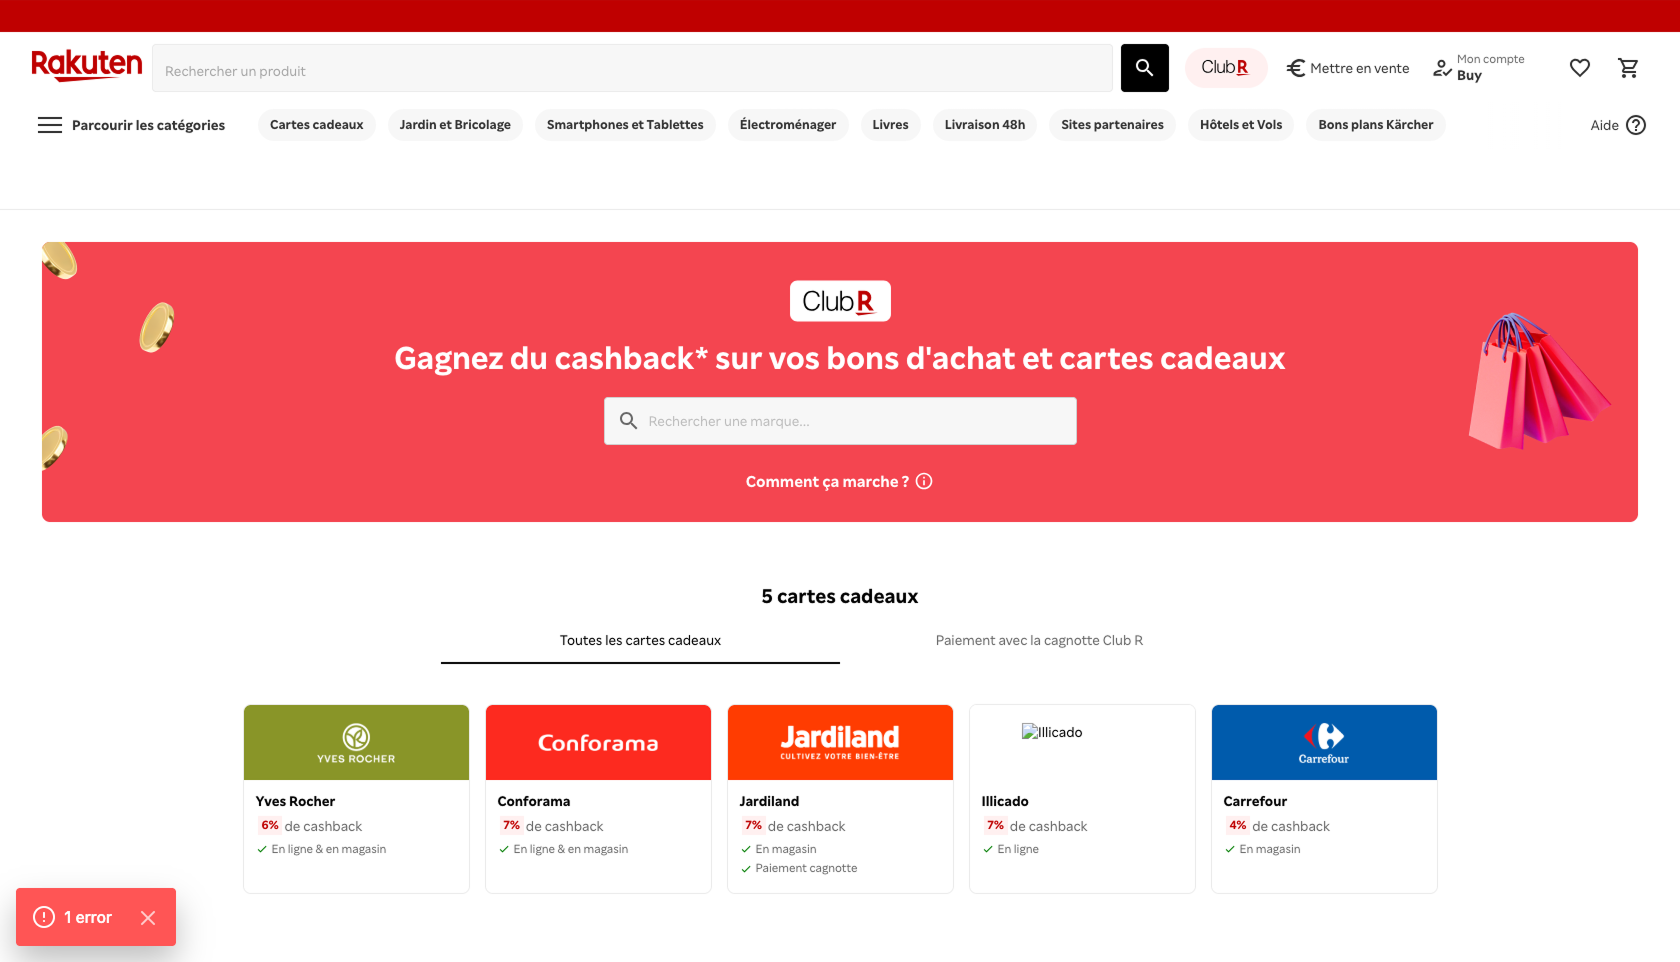
\includegraphics[width=0.95\textwidth]{../assets/dark_mode/buy-fo-gift-card-light.png}
    \caption{Gift card purchase screen displayed in light mode.}
    \label{fig:buy-fo-gift-card-light}
\end{figure}

\begin{figure}[H]
    \centering
    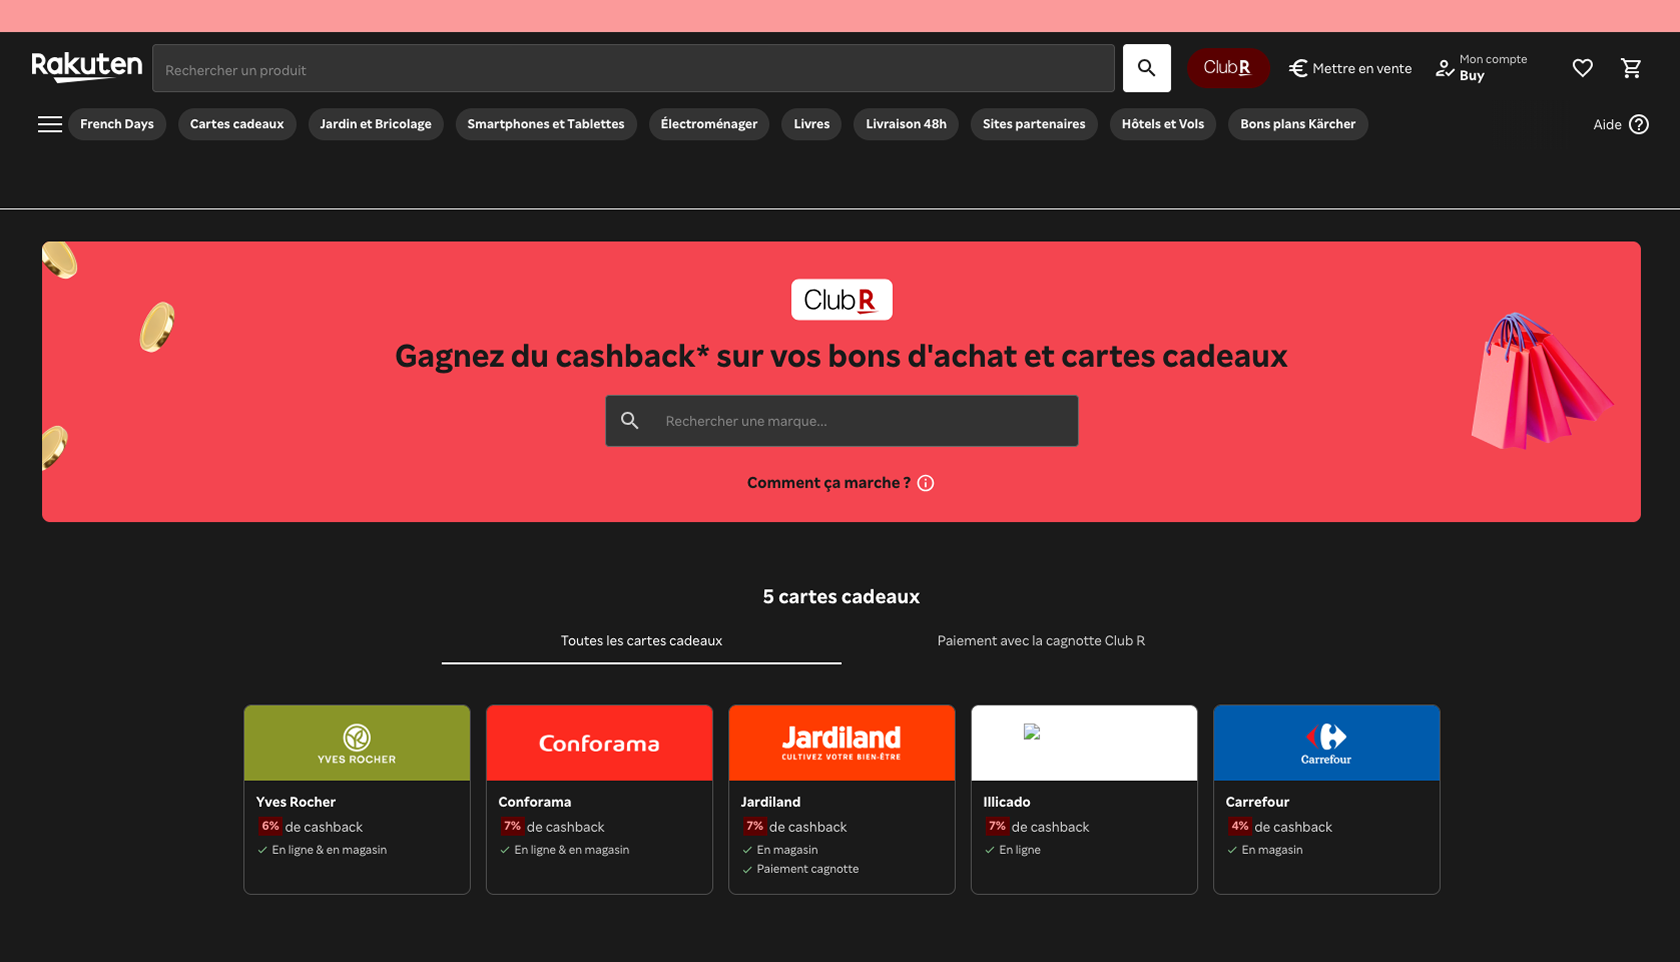
\includegraphics[width=0.95\textwidth]{../assets/dark_mode/buy-fo-gift-card-dark.png}
    \caption{Gift card purchase screen displayed in dark mode.}
    \label{fig:buy-fo-gift-card-dark}
\end{figure}

The following figures present additional screens from different applications
displayed in dark mode. They illustrate the application of the dark theme
across different interfaces and use cases.

\begin{figure}[H]
    \centering
    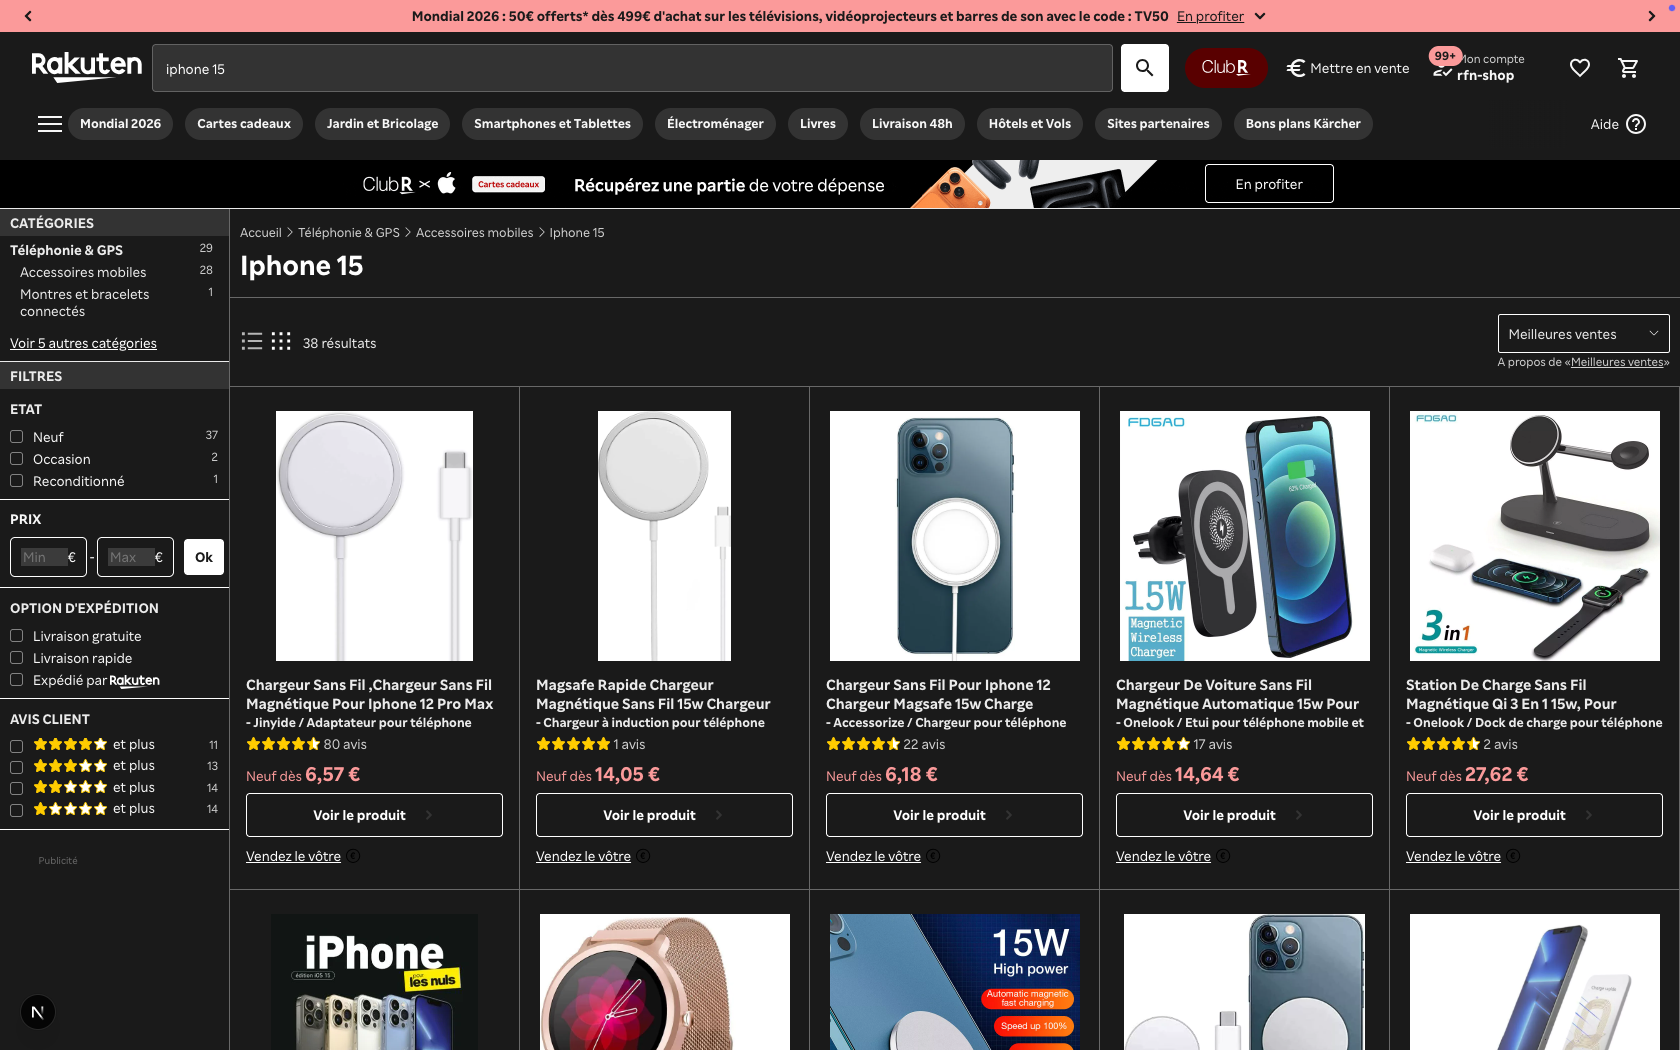
\includegraphics[width=0.95\textwidth]{../assets/dark_mode/vis-fo-products.png}
    \caption{Product listing screen displayed in dark mode.}
    \label{fig:vis-fo-products}
\end{figure}

\begin{figure}[H]
    \centering
    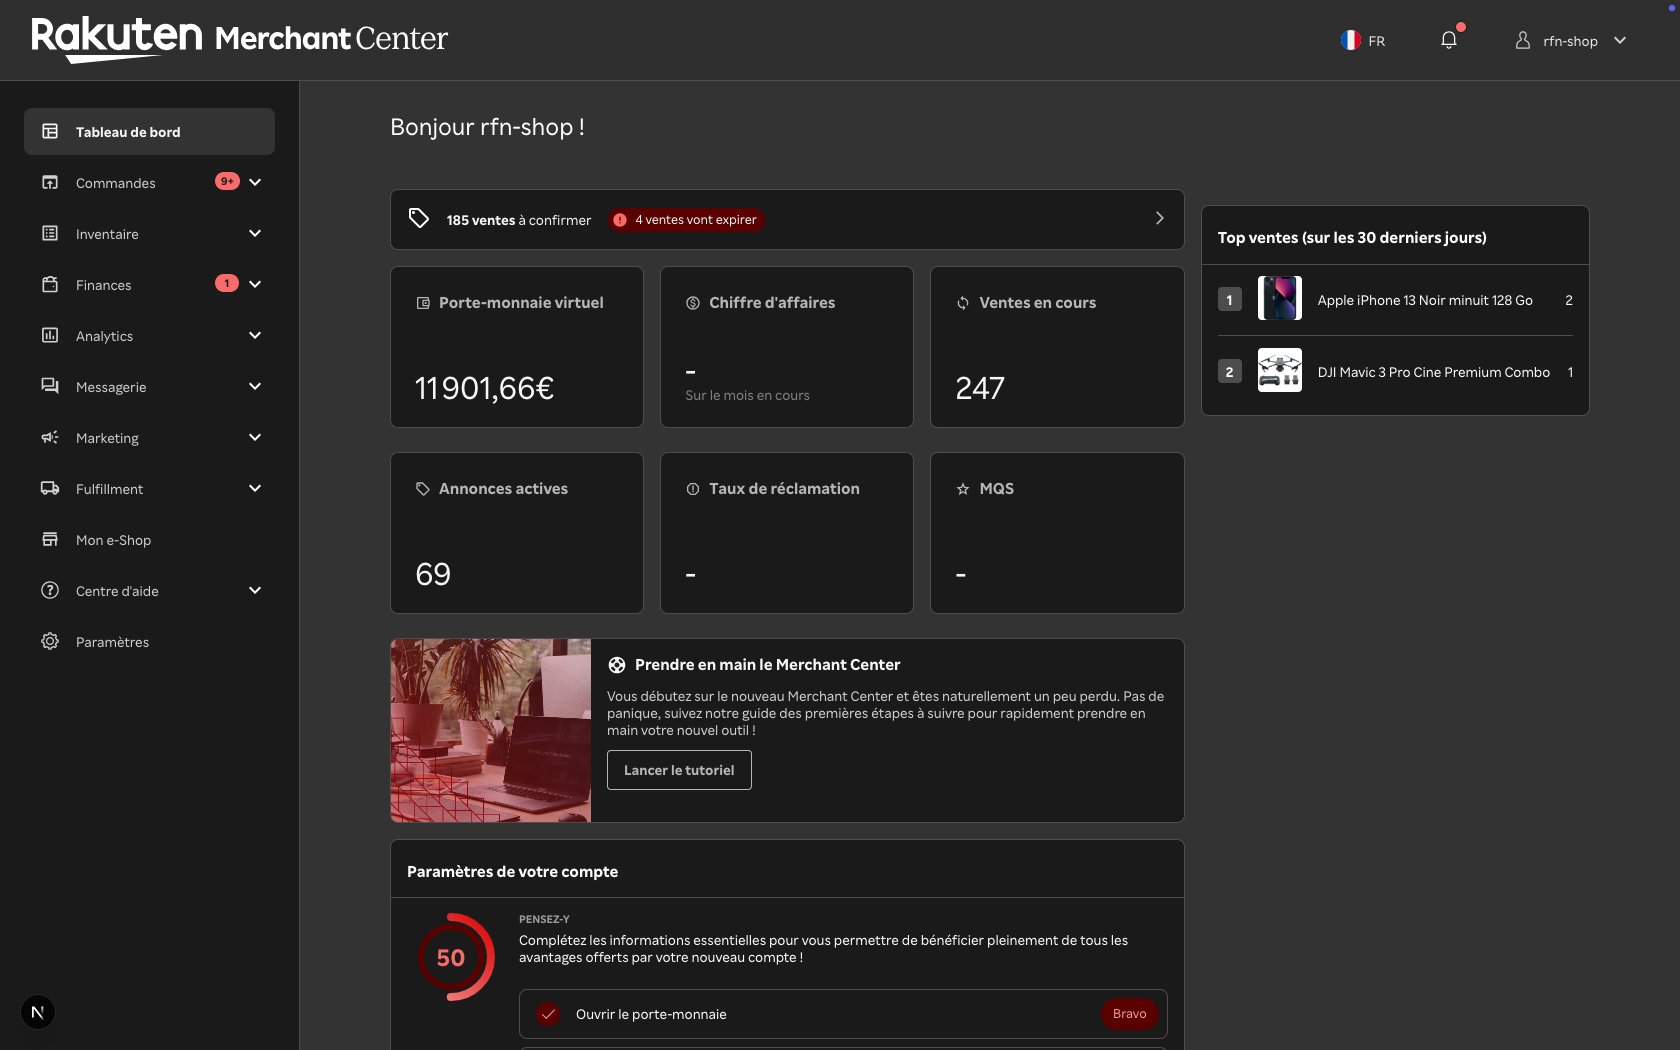
\includegraphics[width=0.95\textwidth]{../assets/dark_mode/b2c-dashboard.png}
    \caption{B2C dashboard displayed in dark mode.}
    \label{fig:b2c-dashboard}
\end{figure}

\section{Conclusion and Future Improvements}

The dark mode implementation established a centralized and reusable foundation across the frontend ecosystem. By introducing shared CSS variables, the \texttt{ThemeContextProvider}, MUI v7 support, and progressive integration into consuming applications, the solution provides a consistent theme management mechanism while reducing duplicated logic. The implementation was also validated through Storybook and Chromatic to ensure visual consistency across both themes.

Although the foundation is fully implemented, several improvements remain possible. Handling transparency with CSS variables could be further improved, visual assets may require additional theme-specific adaptations, and the remaining applications can progressively adopt the shared dark mode infrastructure. Future development should also continue using Storybook and Chromatic to monitor visual regressions and maintain consistency between light and dark themes.

Overall, this work provides a scalable foundation for dark mode across the frontend ecosystem while leaving room for further refinement and progressive adoption.

\clearpage
